%% RSET Project / Seminar LaTex Template Version 1.0 - November 2023

\documentclass[12pt,a4paper,titlepage]{report}

% Page layout
\usepackage[left=2.8cm, right=2.2cm, top=3cm, bottom=2.5cm]{geometry}

% Graphics and figure handling
\usepackage{graphicx}        % for including graphics
\usepackage{float}           % for precise placement of figures and tables
\usepackage{caption}         % for caption adjustments
\usepackage{subcaption}      % for subfigures
\usepackage{tcolorbox}       % for colored boxes
% Mathematical symbols and environments
\usepackage{amsmath}         % for math symbols and environments
\usepackage{amssymb}         % for additional math symbols
\usepackage[T1]{fontenc}  % Better font encoding for special characters
\usepackage{textcomp}     % Provides additional text symbols
% Fonts and symbols
\usepackage{latexsym}        % LASY symbols
\usepackage{eufrak}          % for Fraktur fonts
\usepackage{type1cm}         % scalable fonts
\usepackage{textcomp}
% Other useful packages
\usepackage{longtable}       % for tables that span multiple pages
\usepackage{listings}        % for code listings
\usepackage{xcolor}          % for color support in listings
\usepackage{pdfpages}        % for including PDF pages
\usepackage{url}             % for handling URLs
\usepackage{acro}            % for acronyms
\usepackage{titlesec}        % for section title formatting
\usepackage{listings}
\usepackage{pgfplots}
\usepgfplotslibrary{dateplot}
\pgfplotsset{compat=1.18} 
\usepackage{pgfplotstable}
\lstdefinelanguage{YAML}{
  keywords={true,false,null,y,n},
  keywordstyle=\color{blue}\bfseries,
  basicstyle=\ttfamily\small,
  sensitive=false,
  comment=[l]{\#},
  commentstyle=\color{green}\ttfamily,
  stringstyle=\color{red}\ttfamily,
  morestring=[b]',
  morestring=[b]"
}
\usepackage{color}

\definecolor{dartblue}{RGB}{0,0,255}
\definecolor{dartgreen}{RGB}{0,128,0}
\definecolor{dartred}{RGB}{255,0,0}

\lstdefinelanguage{Dart}{
  keywords={abstract, as, assert, async, await, break, case, catch, class, const, continue, default, deferred, do, dynamic, else, enum, export, extends, factory, false, final, finally, for, get, if, implements, import, in, is, library, new, null, operator, part, rethrow, return, set, static, super, switch, sync, this, throw, true, try, typedef, var, void, while, with, yield},
  keywordstyle=\color{dartblue}\bfseries,
  morecomment=[l]{//},
  morecomment=[s]{/*}{*/},
  morestring=[b]',
  morestring=[b]",
  commentstyle=\color{dartgreen}\ttfamily,
  stringstyle=\color{dartred}\ttfamily,
  identifierstyle=\color{black},
}
% Formatting
\captionsetup{justification=centering}  % Centering captions

% Color and formatting for listings (code)
\lstset{basicstyle=\ttfamily, columns=fullflexible, frame=single, breaklines=true, postbreak=\mbox{\textcolor{red}{$\hookrightarrow$}\space}}

% Example new sectioning titles format (optional)
\titleformat{\section}{\normalfont\Large\bfseries}{\thesection}{1em}{}

% Additional packages if needed
\usepackage{epsfig}          % legacy support for PostScript figures


\definecolor{customgreen}{rgb}{0,0.6,0}
\definecolor{customgray}{rgb}{0.5,0.5,0.5}
\definecolor{custommauve}{rgb}{0.6,0,0.8}
\lstdefinelanguage{HTML}{
	sensitive=true,
	keywords={},
	otherkeywords={<, >, /},
	morecomment=[s]{<!--}{-->},
	morestring=[b]"
}


\lstset{ 
	basicstyle=\small,        % the size of the fonts that are used for the code
	breaklines=true,                 % sets automatic line breaking
	commentstyle=\color{customgreen},    % comment style
	firstnumber=1,                % start line enumeration with line 1000
	frame=single,	                   % adds a frame around the code
	keepspaces=true,                 % keeps spaces in text, useful for keeping indentation of code (possibly needs columns=flexible)
	keywordstyle=\color{blue},       % keyword style
	numbers=left,                    % where to put the line-numbers; possible values are (none, left, right)
	numbersep=10pt,                   % how far the line-numbers are from the code
	numberstyle=\tiny\color{customgray}, % the style that is used for the line-numbers
	rulecolor=\color{black},         % if not set, the frame-color may be changed on line-breaks within not-black text (e.g. comments (green here))
	showspaces=false,                % show spaces everywhere adding particular underscores; it overrides 'showstringspaces'
	showstringspaces=false,          % underline spaces within strings only
	showtabs=false,                  % show tabs within strings adding particular underscores
	stepnumber=1,                    % the step between two line-numbers. If it's 1, each line will be numbered
	stringstyle=\color{custommauve},     % string literal style
	tabsize=2,	                   % sets default tabsize to 2 spaces
	title=\lstname                   % show the filename of files included with \lstinputlisting; also try caption instead of title
}


\titleformat{\chapter}[display]
{\normalfont\Large\bfseries\centering}{\chaptertitlename\
	\thechapter}{25pt}{\Large}
\titleformat{\section}{\normalfont\bfseries}{\noindent\thesection}{20pt}{}
\titleformat{\subsection}{\normalfont\small\bfseries}{\thesubsection}{15pt}{\small}
\titlespacing*{\chapter}{0pt}{0pt}{40pt}


\begin{document}
\titlepage
\thispagestyle{empty}
\begin{center}
	
\includegraphics[scale=0.35]{Figures/logo1.png}\\[0.2cm]
	\large \textit{Project Phase II Report On}\\[0.3cm]
	\Large \textbf{Advanced Supply and Trade Resource Optimisation (A.S.T.R.O.)}\\[0.3cm]
	\textit{Submitted in partial fulfillment of the
		requirements for the award of the degree of}\\[0.3cm]
	{\huge {$\mathfrak {Bachelor\; of\; Technology}$}}\\[.3cm]
	%{\Large {$\mathfrak {In}$}}\\[.5cm]
	%{\Large {$\mathfrak {Computer\; Science\; \&\; Engineering}$}}\\[2cm]
	\textit{in}\\[.2cm]
	{\Large \bf \itshape{{Computer Science and Business Systems}}}\\[0.7cm]
	\large \bfseries{By}\\[.1cm]
	\large \bfseries{Amel Chandra (U2109009)}\\[0.2cm]
	\large \bfseries{Bharath S. (U2109018)}\\[0.2cm]
	\large \bfseries{Joepaul Vilsan (U2109033)}\\[0.2cm]
	\large \bfseries{Shane George Salphie (U2109063)}\\[0.2cm]
	\large \bfseries{Under the guidance of}\\[0.3cm]
	\large \bfseries{Dr. Nikhila T. Bhuvan}\\[0.2cm]
	%		\includegraphics[width=8.0cm]{logo (1).jpg}\\[0.5cm]
	\large \textbf{Department of Computer Science and Business Systems}\\
	\large \textbf{Rajagiri School of Engineering \&\ Technology (Autonomous)}\\
	\small \bfseries{(Parent University: APJ Abdul Kalam Technological University)}\\
	\large \textbf{Rajagiri Valley, Kakkanad, Kochi, 682039}\\[0.2cm]
	\large \bfseries{April 2025}
\end{center}

\newpage
\thispagestyle{empty}
\vspace{1cm}
\begin{center}
	%	\textbf {DEPARTMENT OF COMPUTER SCIENCE \&\ ENGINEERING}\\
	%	\small \textbf{RAJAGIRI SCHOOL OF ENGINEERING \&\ TECHNOLOGY (AUTONOMOUS)}\\

	%	\small \textbf{RAJAGIRI VALLEY, KAKKANAD, KOCHI, 682039}\\
	%   \small \bfseries{(Affiliated to APJ Abdul Kalam Technological University)}\\[0.5cm]
	%\begin{figure}[htbp]
	%	\centering
	%\includegraphics[scale=0.40]{logo (1).jpg}
	%   \includegraphics[width=8.0cm]{logo (1).jpg}\\[0.5cm]
	%\end{figure}
	\large \bfseries{\huge{CERTIFICATE}}\\[1cm]
\end{center}

\renewcommand{\baselinestretch}{1.2}\normalsize

\sloppy
\emph{This is to certify that the project report entitled \textbf{”Advanced Supply and Trade Resource Optimisation”} is a bonafide record of the work done by \textbf{\mbox{Amel Chandra} (U2109009), \mbox{Bharath S (U2109018)}, \mbox{Joepaul Vilsan (U2109033)}, \mbox{Shane} \mbox{George} \mbox{Salphie (U2109063)}}, submitted to the Rajagiri School of Engineering \& Technology (RSET) (Autonomous) in partial fulfillment of the requirements for the award of the degree of Bachelor of Technology (B. Tech.) in "Computer Science and Business Systems" during the academic year 2024-2025.}\\[2.5cm]

\begin{flushleft}


	\begin{longtable}{p{5.8cm} p{5.8cm} p{5.8cm}}
		{Dr. Nikhila T. Bhuvan} & {Mr. Mahesh K.M.}      & {Dr. Divya James}     \\
		{Project Guide}         & {Project Co-ordinator} & {Head Of Department}  \\
		{Associate Professor}   & {Assistant Professor}  & {Associate Professor} \\
		{Dept. of CU}           & {Dept. of CU}          & {Dept. of CU}         \\
		{RSET}                  & {RSET}                 & {RSET}                \\
	\end{longtable}
\end{flushleft}
\vspace{2cm}






\renewcommand{\baselinestretch}{1.5}\normalsize
\newpage
%\renewcommand\abstractname{ACKNOWLEDGEMENTS}
\chapter*{ACKNOWLEDGMENT}
%\begin{abstract}
\pagenumbering{roman}
\setcounter{page}{1}
\addcontentsline{toc}{chapter}{Acknowledgment}
\vspace{1.5cm}
%\begin{spacing}{}
\paragraph\ We wish to express my sincere gratitude towards \textbf{Rev. Dr. Jaison Paul Mulerikkal}, Principal of RSET, and \textbf{Dr. Divya James}, Head of the Department of Computer Science and Business Systems for providing us with the opportunity to undertake my project, \textbf{"Advanced Supply and Trade Resource Optimisation"}.
\paragraph\ We are highly indebted to our project coordinators, \textbf{Dr. Nikhila T Bhuvan}, Associate Professor, Department of Computer Science and Business Systems, \textbf{Ms. Ancy C A}, Assistant Professor, Department of Computer Science and Business Systems,\textbf{Mr. Mahesh K M} Assistant Professor,Department of Computer Science and Business Systems for their valuable support.

\paragraph\ It is indeed my pleasure and a moment of satisfaction for me to express my sincere
gratitude to my project guide \textbf{Dr. Nikhila T Bhuvan} for her patience and all the priceless advice and wisdom she has shared with me.
\paragraph\ Last but not the least, I would like to express my sincere gratitude towards all other teachers and friends for their continuous support and constructive ideas.
%\end{spacing}
\begin{flushright}
	\textbf{Amel Chandra}\\
	\textbf{Bharath S}\\
	\textbf{Joepaul Vilsan}\\
	\textbf{Shane George Salphie}
\end{flushright}


\newpage

\renewcommand{\baselinestretch}{1.5}\normalsize

\chapter*{Abstract}
\addcontentsline{toc}{chapter}{Abstract}
\vspace{1.5cm}
\paragraph{}\ \ \ \ Small-scale vendors face significant challenges in competing with large retail chains due to limited purchasing power, inefficient logistics, and restricted access to financial services. These barriers often hinder their ability to manage demand fluctuations and make informed business decisions, threatening their long-term sustainability. This project aims to address these issues by developing a comprehensive platform that empowers small vendors through collaborative purchasing, optimized logistics, and data-driven decision-making. By enabling vendors to combine orders, the platform facilitates bulk purchasing, unlocking competitive discounts and cost savings. Advanced algorithms optimize logistics by streamlining delivery routes, thereby reducing transportation costs and enhancing operational efficiency.  These features empower vendors to make strategic decisions that align with market demands and their business goals. The ultimate goal is to level the playing field for small vendors, enabling them to compete effectively with larger retail chains while fostering sustainable growth in local economies. The deliverables of this project include a fully functional platform supporting vendor collaboration and an optimized logistics module to reduce operational costs. By promoting economic resilience, enhancing competitiveness, and driving sustainable development, this project seeks to strengthen the local vendor ecosystem and contribute to the overall development of communities.

%\end{spacing}
%\end{abstract}


\newpage
\normalsize{}

%\pagenumbering{roman}
%\setcounter{page}{4}
%\begin{spacing}{}
\tableofcontents
%\end{spacing}
% \thispagestyle{empty}
\newpage

\chapter*{List of Abbreviations}
\addcontentsline{toc}{chapter}{List of Abbreviations}

ASTRO - Advanced Supply and Trade Resource Optimisation \\
SDG - Sustainable Development Goals \\
API - Application Programming Interface \\
ACO - Ant Colony Optimisation \\
GA - Genetic Algorithm \\
SME - Small to Medium-sized Enterprises \\
UI - User Interface \\
MOQ - Minimum Order Quantity \\
EAGA - Environment Adaptive Genetic Algorithm \\
EAACO - Environment Adaptive Ant Colony Optimisation \\
DBSCAN - Density-Based Spatial Clustering of Applications with Noise \\
KNN - K-Nearest Neighbours \\

\newpage

\listoffigures
\addcontentsline{toc}{chapter}{List of Figures}
% \thispagestyle{empty}
\newpage


% \pagenumbering{roman}
%\setcounter{page}{9}
\listoftables
\addcontentsline{toc}{chapter}{List of Tables}
%	\addcontentsline{toc}{chapter}{List of Abbreviations}
%	\listof{Abbreviations}
% \thispagestyle{empty}
\newpage



\cleardoublepage

\pagenumbering{arabic}
\setcounter{page}{1}

\chapter{Introduction}

Small-scale vendors are essential contributors to local economies, offering unique products and
personalized services that enrich communities. However, they face significant challenges
competing against large retail chains, which benefit from greater purchasing power, efficient
logistics, and easier access to financial resources. Due to limited resources, small vendors often
struggle with high supply costs, fragmented logistics, and restricted access to credit, hindering
their ability to grow and compete effectively.
The ASTRO (Advanced Supply and Trade Resource Optimization) platform addresses these
challenges by providing a comprehensive solution that empowers small vendors through
collaborative purchasing, logistics optimization, and data-driven financial services. By allowing
vendors to pool orders, ASTRO enables them to achieve bulk pricing similar to large retailers,
reducing per-unit costs and enhancing profitability. The platform also incorporates advanced
logistics optimization algorithms, improving delivery efficiency and reducing operational
expenses. Additionally, ASTRO offers financial services based on transaction data, enabling
vendors to access credit and make informed decisions for business expansion.

ASTRO’s functionality extends further with real-time demand forecasting tools, equipping
vendors with predictive insights that help manage inventory and adapt to changing market
demands. Through these features, ASTRO not only improves individual vendor competitiveness
but also fosters economic resilience in local communities by supporting sustainable growth and
operational efficiency. As a result, ASTRO is positioned as a vital resource for small vendors,
helping them navigate a competitive retail landscape while contributing to the stability and
diversity of local economies.
\section{Background}

Small-scale vendors are integral to the fabric of local economies, providing unique products,
personalized services, and fostering vibrant community interactions that larger retail chains
often cannot replicate. These vendors contribute significantly to economic diversity, cultural
richness, and employment within their communities. However, despite their crucial role,
small-scale vendors face persistent challenges that impede their ability to compete effectively
with larger retail entities. These challenges include limited purchasing power, inefficient logistics,
restricted access to financial services, and a lack of data-driven decision-making tools.
In today’s highly competitive retail landscape, large retail chains leverage economies of scale to
negotiate bulk purchasing discounts, implement sophisticated logistics networks, and utilize
advanced data analytics to optimize their operations and marketing strategies. In contrast,
small-scale vendors typically operate with constrained resources, making it difficult for them to
achieve similar efficiencies and cost-effectiveness. This disparity not only affects their
profitability but also limits their capacity to respond to market fluctuations and evolving
consumer demands.
The ASTRO platform (Advanced Supply and Trade Resource Optimization) is designed to
address these disparities by providing small-scale vendors with tools and services that enhance
their competitive edge. By enabling collaborative purchasing, optimizing logistics, and offering
data-driven financial services, ASTRO empowers local vendors to achieve bulk pricing,
streamline their operations, and make informed business decisions. This platform aims to bridge
the gap between small vendors and large retail chains, fostering economic resilience and
sustainable growth within local communities.
Moreover, the advent of digital transformation has revolutionized various industries, including
retail. The integration of technology into traditional business models is essential for small-scale
vendors to remain relevant and competitive. ASTRO leverages modern technological
advancements, such as machine learning algorithms for logistics optimization and predictive
analytics for demand forecasting, to deliver practical solutions tailored to the specific needs of
small vendors. The significance of ASTRO extends beyond individual business success; it
contributes to the overall economic health of communities by supporting the sustainability and
growth of small-scale enterprises.

\section{Problem Definition}

Small-scale vendors face a significant challenge in today’s competitive retail landscape, where large retail chains dominate with bulk pricing, advanced logistics, and extensive resources. This disparity puts small vendors at a disadvantage, as they often lack the economies of scale and infrastructure necessary to compete effectively. The problem is that, despite being crucial to local economies, small vendors struggle with high operational costs, inefficient logistics, and limited access to affordable credit, all of which hinder their ability to grow sustainably. This issue is exacerbated by the lack of platforms that cater to the specific needs of small-scale businesses, especially when it comes to aggregating demand, optimizing supply chains, and improving cash flow.

Without access to bulk purchasing and efficient logistics, small vendors pay higher prices for goods, limiting their profit margins and making it difficult to reinvest in their businesses. Furthermore, the absence of accurate demand forecasting and inventory management tools leads to overstocking or stockouts, reducing customer satisfaction and revenue. These issues underscore the need for a system that enables small vendors to pool their purchasing power, streamline their supply chains, and make data-driven decisions to improve their competitiveness.

The Advanced Supply and Trade Resource Optimization (A.S.T.R.O.) platform seeks to address this gap by providing small-scale vendors with the tools to compete with larger retail chains. A.S.T.R.O. enables collaborative purchasing, allowing vendors to aggregate their orders and access bulk discounts, thus reducing product costs. Additionally, the platform offers real-time demand forecasting, helping vendors optimize inventory levels to avoid both overstock and stockouts. To address financial limitations, A.S.T.R.O. includes data-driven financial services, such as credit assessment and tailored loans, designed to enhance cash flow and support business growth.

By facilitating these services, A.S.T.R.O. aims to foster economic resilience and sustainable growth in local communities. Its focus on empowering small vendors with advanced tools levels the playing field, promoting a more equitable and competitive market environment. This approach not only ensures that small vendors can thrive but also contributes to the overall health and diversity of the retail ecosystem.

\section{Scope and Motivation}
The ASTRO platform is a multifaceted solution designed to support small-scale vendors by addressing key operational challenges through technological integration and collaborative strategies. The scope of ASTRO encompasses the development and implementation of several core functionalities:

\begin{enumerate}
	\item \textbf{Collaborative Purchasing:} ASTRO facilitates group purchasing among small vendors, allowing them to pool their orders to achieve bulk pricing discounts. This feature enhances purchasing power, enabling vendors to reduce their cost of goods sold and improve profit margins.

	\item \textbf{Logistics Optimization:} Utilizing advanced algorithms, ASTRO optimizes delivery routes to reduce transportation costs and improve delivery efficiency. By streamlining logistics, the platform helps vendors achieve timely deliveries and minimize operational expenses.

	\item \textbf{Real-Time Demand Forecasting:} Leveraging predictive analytics, ASTRO provides real-time demand forecasting tools that help vendors anticipate market demand and manage inventory levels effectively. Accurate demand forecasting reduces the risk of overstocking or stockouts, ensuring that vendors can meet customer needs efficiently.

	\item \textbf{User-Friendly Interface:} ASTRO is designed with an intuitive user interface that ensures ease of use for vendors with varying levels of technical expertise. This feature maximizes user engagement and ensures that vendors can effectively utilize the platform’s functionalities to enhance their business operations.
\end{enumerate}

The motivation behind ASTRO stems from the urgent need to empower small-scale vendors in an increasingly competitive retail environment. As large retail chains continue to dominate the market through superior purchasing power and advanced logistics, small vendors risk marginalization and potential business failure. ASTRO addresses these challenges by providing a robust platform that enhances operational efficiency, reduces costs, and increases access to financial resources, thereby enabling small vendors to compete on a more equal footing.

Additionally, ASTRO is motivated by the broader goal of fostering economic resilience and sustainability within local communities. Small-scale vendors are pivotal to the economic diversity and vitality of local markets, contributing to job creation and community development. By supporting these vendors, ASTRO not only enhances individual business success but also strengthens the overall economic fabric of communities, promoting long-term sustainable growth and economic stability.
\section{Objectives}
The ASTRO project is guided by a set of clear and actionable objectives aimed at addressing the challenges faced by small-scale vendors. These objectives are designed to enhance operational efficiency, reduce costs, and provide financial support, thereby empowering vendors to compete effectively in the marketplace. The primary objectives of ASTRO include:

\begin{enumerate}
	\item \textbf{Enable Collaborative Purchasing:}
	      \begin{itemize}
		      \item \textbf{Objective:} Develop a robust system that allows small vendors to combine their orders, thereby achieving bulk purchasing discounts.
		      \item \textbf{Outcome:} Increased purchasing power, reduced cost of goods sold, and improved profit margins for vendors.
	      \end{itemize}

	\item \textbf{Optimize Logistics:}
	      \begin{itemize}
		      \item \textbf{Objective:} Implement advanced route optimization algorithms to streamline delivery processes, reduce transportation costs, and enhance operational efficiency.
		      \item \textbf{Outcome:} Cost-effective logistics operations, timely deliveries, and reduced operational expenses.
	      \end{itemize}

	\item \textbf{Provide Real-Time Demand Forecasting:}
	      \begin{itemize}
		      \item \textbf{Objective:} Integrate predictive analytics tools to offer real-time demand forecasting, enabling vendors to anticipate market demand and manage inventory levels effectively.
		      \item \textbf{Outcome:} Minimization of overstocking and stockouts, improved inventory management, and enhanced ability to meet customer demands.
	      \end{itemize}


	\item \textbf{Promote Economic Resilience and Sustainability:}
	      \begin{itemize}
		      \item \textbf{Objective:} Foster economic resilience by providing small vendors with the tools and resources needed to sustain and grow their businesses.
		      \item \textbf{Outcome:} Long-term sustainability, increased competitiveness, and strengthened economic stability within local communities.
	      \end{itemize}

	\item \textbf{Enhance User Experience and Accessibility:}
	      \begin{itemize}
		      \item \textbf{Objective:} Design a user-friendly interface that ensures easy access to the platform’s features, regardless of vendors’ technical expertise.
		      \item \textbf{Outcome:} High user engagement, effective utilization of platform functionalities, and improved overall user satisfaction.
	      \end{itemize}

	\item \textbf{Support Community Development:}
	      \begin{itemize}
		      \item \textbf{Objective:} Encourage collaboration and mutual support among vendors, fostering a sense of community and shared growth.
		      \item \textbf{Outcome:} Collective bargaining power, knowledge sharing, and resource optimization, leading to a stronger and more cohesive vendor network.
	      \end{itemize}
\end{enumerate}

By achieving these objectives, ASTRO aims to create a comprehensive solution that empowers small-scale vendors to overcome their operational challenges, enhance their competitiveness, and contribute to the sustainable growth of local economies. Each objective is strategically aligned to address specific pain points, ensuring that the platform delivers tangible benefits and drives meaningful improvements in vendors' business operations.




\section{Relevance}

The relevance of the ASTRO project is multifaceted, addressing critical needs within the retail ecosystem and contributing to broader economic and social goals. Key aspects of ASTRO’s relevance include:

\begin{enumerate}
	\item \textbf{Economic Empowerment of Small Vendors:}
	      \begin{itemize}
		      \item \textbf{Impact:} ASTRO directly addresses the economic challenges faced by small-scale vendors, enhancing their purchasing power and optimizing logistics cost. This empowerment enables vendors to operate more efficiently, reduce costs, and increase profitability, thereby improving their economic standing and sustainability.
	      \end{itemize}

	\item \textbf{Enhancing Local Economies:}
	      \begin{itemize}
		      \item \textbf{Impact:} By supporting small vendors, ASTRO contributes to the vitality and resilience of local economies. Small businesses are integral to economic diversification and job creation, promoting the long-term sustainability of local markets.
	      \end{itemize}

	\item \textbf{Technological Advancement and Digital Transformation:}
	      \begin{itemize}
		      \item \textbf{Impact:} ASTRO exemplifies the role of technology in transforming traditional business models. By leveraging advanced algorithms for logistics optimization, predictive analytics for demand forecasting, ASTRO introduces modern technological solutions to enhance the operational capabilities of small vendors. This digital transformation is crucial for small businesses to remain competitive in an increasingly digital and data-driven marketplace.
	      \end{itemize}

	\item \textbf{Sustainable Growth and Environmental Impact:}
	      \begin{itemize}
		      \item \textbf{Impact:} ASTRO’s logistics optimization not only reduces operational costs but also minimizes the environmental footprint of delivery processes. By streamlining routes and reducing transportation distances, ASTRO contributes to more sustainable business practices, aligning with global efforts to reduce carbon emissions and promote environmental sustainability.
	      \end{itemize}
	\item \textbf{Competitive Parity:}
	      \begin{itemize}
		      \item \textbf{Impact:} ASTRO helps small vendors achieve competitive parity with larger retail chains by providing tools that enhance their operational efficiency and cost-effectiveness. This parity is crucial for maintaining market diversity and preventing the monopolistic dominance of large retailers, ensuring a healthy and competitive marketplace that benefits both vendors and consumers.
	      \end{itemize}

	\item \textbf{Adaptation to Market Trends:}
	      \begin{itemize}
		      \item \textbf{Impact:} In a rapidly evolving retail environment, the ability to adapt to changing market trends and consumer behaviors is essential. ASTRO’s real-time demand forecasting and data-driven insights enable small vendors to stay ahead of market trends, respond promptly to consumer needs, and adapt their inventory and marketing strategies accordingly.
	      \end{itemize}

	\item \textbf{Community Building and Collaboration:}
	      \begin{itemize}
		      \item \textbf{Impact:} ASTRO fosters a collaborative ecosystem where small vendors can work together to achieve common goals. This sense of community and mutual support enhances collective bargaining power, knowledge sharing, and resource optimization, contributing to the overall strength and cohesion of the local vendor network.
	      \end{itemize}

	\item \textbf{Scalability and Replicability:}
	      \begin{itemize}
		      \item \textbf{Impact:} ASTRO’s platform is designed to be scalable, allowing it to be replicated in various regions and adapted to different market conditions. This scalability ensures that the platform can benefit a wide range of small-scale vendors across different industries, promoting widespread economic empowerment and community resilience.
	      \end{itemize}

	\item \textbf{Support for Economic Diversity and Stability:}
	      \begin{itemize}
		      \item \textbf{Impact:} By enabling small vendors to thrive, ASTRO supports economic diversity, which is essential for the stability and resilience of local economies. Diverse economic activities reduce dependence on a single sector or large corporations, making communities more adaptable to economic shocks and changes.
	      \end{itemize}

	\item \textbf{Promoting Entrepreneurship and Innovation:}
	      \begin{itemize}
		      \item \textbf{Impact:} ASTRO encourages entrepreneurship by lowering the barriers to entry for small vendors. By providing the necessary tools and resources, ASTRO enables aspiring entrepreneurs to start and grow their businesses, fostering a culture of innovation and economic dynamism within local communities.
	      \end{itemize}

	\item \textbf{Enhanced Customer Experience:}
	      \begin{itemize}
		      \item \textbf{Impact:} By improving operational efficiency and reducing costs, ASTRO enables small vendors to offer better pricing and more reliable services to their customers. Enhanced customer experiences lead to increased customer loyalty and satisfaction, driving repeat business and positive word-of-mouth referrals.
	      \end{itemize}

	\item \textbf{Economic Resilience and Crisis Management:}
	      \begin{itemize}
		      \item \textbf{Impact:} ASTRO equips small vendors with the tools to better manage economic fluctuations and crises. By optimizing inventory levels, forecasting demand accurately, and accessing financial support, vendors are better prepared to navigate economic downturns, supply chain disruptions, and other unforeseen challenges.
	      \end{itemize}

	\item \textbf{Alignment with Sustainable Development Goals (SDGs):}
	      \begin{itemize}
		      \item \textbf{Impact:} ASTRO aligns with several United Nations Sustainable Development Goals, including Decent Work and Economic Growth (SDG 8), Industry, Innovation, and Infrastructure (SDG 9), and Reduced Inequalities (SDG 10). By empowering small vendors, ASTRO contributes to inclusive and sustainable economic growth, technological innovation, and the reduction of economic disparities.
	      \end{itemize}

	\item \textbf{Enhancing Vendor Autonomy and Empowerment:}
	      \begin{itemize}
		      \item \textbf{Impact:} ASTRO empowers small vendors by giving them greater control over their purchasing, logistics, and financial decisions. This autonomy fosters a sense of ownership and confidence among vendors, encouraging them to take proactive steps towards business improvement and growth.
	      \end{itemize}
\end{enumerate}



\chapter{System Architecture}



\noindent Figure 3.1 illustrates the system architecture for the ASTRO Platform, designed to support small-scale vendors by facilitating bulk order discounts, demand forecasting, and logistics optimisation. This architecture provides a clear overview of the platform’s components and how they work together to streamline the entire process from order initiation to optimized delivery. Here’s a breakdown of the key aspects and importance of this architecture:

\begin{figure}[h]
    \centering
    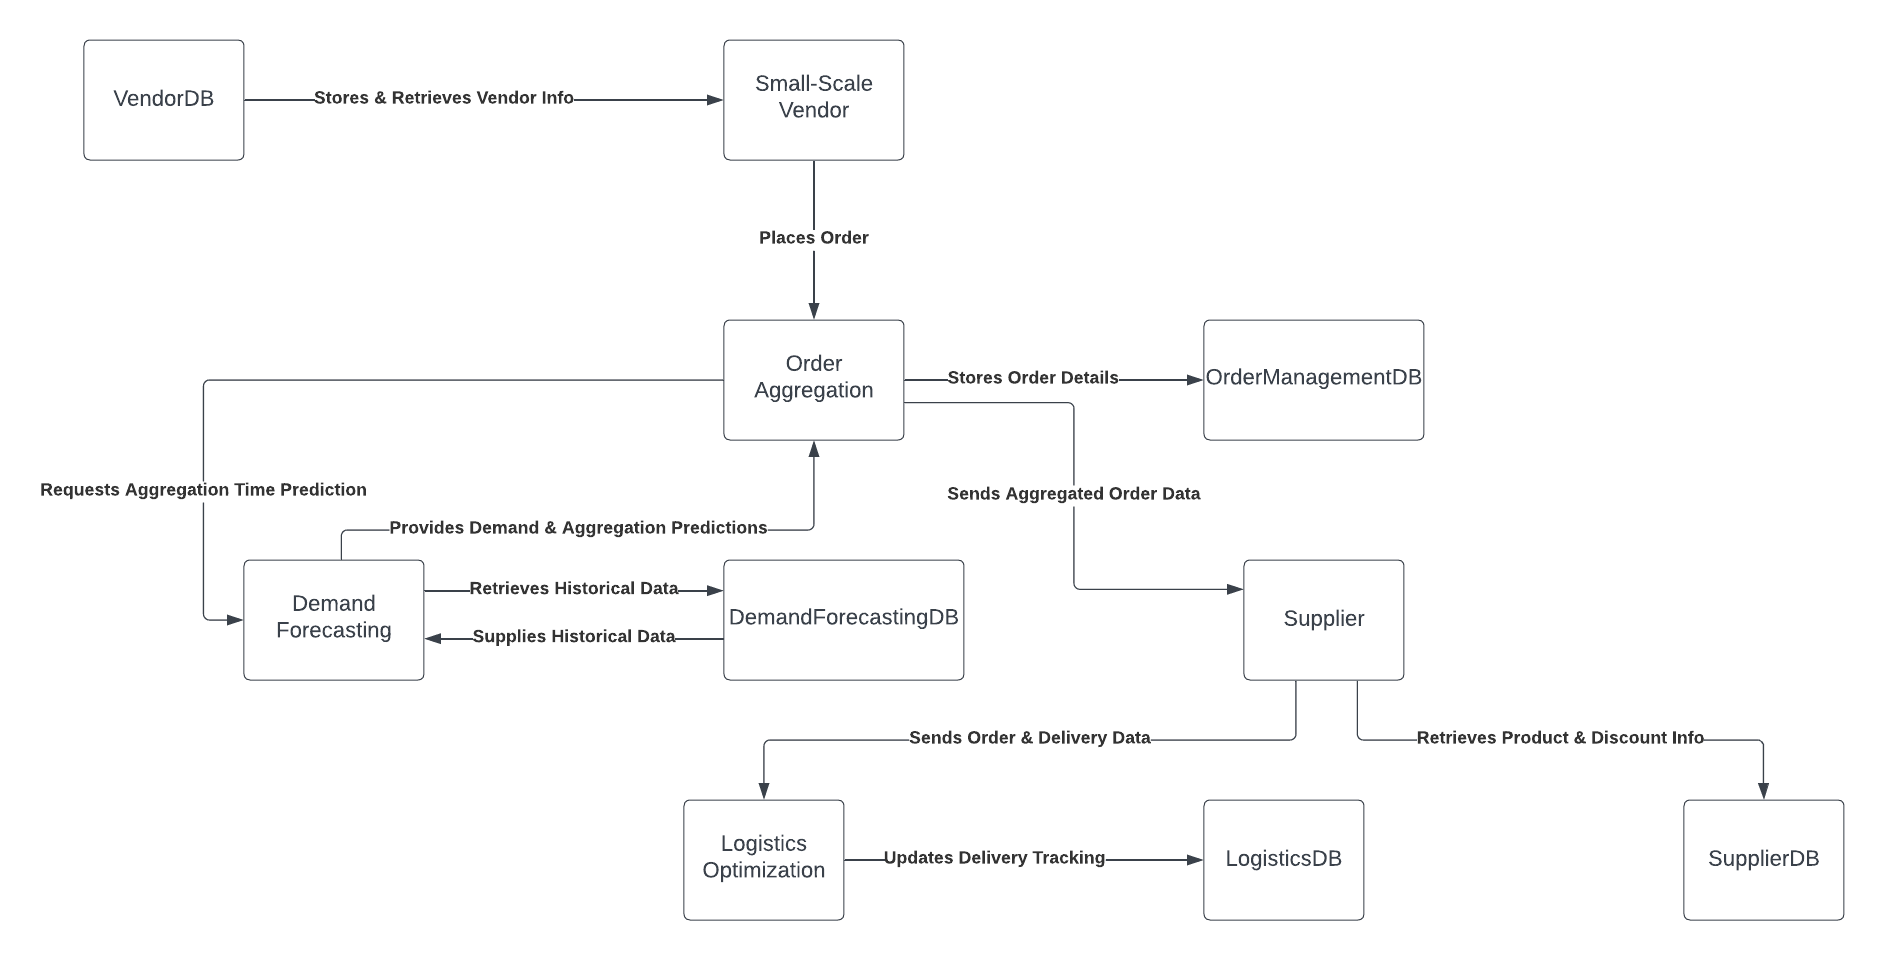
\includegraphics[width=\textwidth]{Figures/system_archh.png}
    \caption{System Architecture}
    \label{fig:architecture}
\end{figure}


\begin{enumerate}
    \item \textbf{High-Level Overview:} The architecture serves as a roadmap, showing the main stages of the platform’s workflow. From initial product viewing and order placement by vendors, through demand forecasting, order aggregation, and logistics optimisation, this high-level overview provides all stakeholders—including vendors, suppliers, and platform administrators—with a clear understanding of the system’s core functionality.

    \item \textbf{Clarifies Data Flow:} The architecture clarifies the flow of data within the system, beginning with the acquisition of order and sales data. This data undergoes preprocessing and feature extraction, followed by demand forecasting with the Neural Prophet model. The forecast data then flows into the Order Aggregation module, which combines vendor orders to meet bulk purchase thresholds. Finally, optimized delivery routes are created through the Logistics Optimisation module, using Green Routing techniques. This sequential data flow enhances system transparency and makes it easy to identify potential bottlenecks.

    \item \textbf{Enables Collaborative Order Aggregation:} The architecture highlights how order aggregation enables small-scale vendors to achieve bulk discounts. By aggregating orders from multiple vendors, the platform ensures Minimum Order Quantities (MOQs) are met, enabling vendors to access bulk discounts typically reserved for larger chains. This aspect of the system is crucial for enhancing the competitiveness of small vendors.

    \item \textbf{Supports Logistics Optimisation through Green Routing:} The architecture emphasizes the logistics optimisation approach used in the platform. The Green Routing component incorporates route flexibility and service time windows to create efficient and environmentally friendly delivery routes. This optimisation minimizes transportation costs and enhances delivery reliability for vendors, contributing to a streamlined and cost-effective supply chain.

    \item \textbf{Enables Real-Time Notifications and Updates:} The system architecture includes a notification mechanism that provides real-time updates to vendors on order status, inventory levels, and logistics. These notifications foster transparency, enabling vendors to make informed decisions about inventory and delivery schedules.

    \item \textbf{Facilitates Collaboration and Communication Among Stakeholders:} The system architecture acts as a shared framework, providing a common language for platform users, developers, and suppliers. It allows stakeholders to better understand the interactions between components and collaborate effectively toward improving platform functionality. This collaborative framework is essential for ensuring smooth operations and adapting to vendor needs.

\end{enumerate}

\noindent Overall, the system architecture is crucial for understanding the ASTRO Platform. It provides a clear visual representation of the platform’s workflow, highlighting key features such as order aggregation, demand forecasting, logistics optimisation, and real-time notifications. These components work together to enhance vendor competitiveness by offering cost-saving opportunities, efficient delivery solutions, and improved collaboration with suppliers.

\section{Dataset}


\textbf{Purpose:} This dataset supports research in sales forecasting, specifically at the item and store levels. The objective is to predict the next three months of sales for individual items at various store locations, applicable for demand forecasting, inventory management, and sales optimisation.

\textbf{Data Collection:} This dataset was collected from multiple store locations, representing real-world sales data with variations in store performance and item demand. It provides diverse daily sales records for individual items across different stores, enabling demand pattern analysis.

\textbf{Data Fields:}
\begin{description}
    \item[\textbf{date:}] Date of each sale record. There are no adjustments for holidays or store closures, simplifying the analysis but possibly requiring external data for event-based effects.
    \item[\textbf{store:}] A unique identifier for each store, allowing for store-level analysis and capturing unique characteristics and item demand differences.
    \item[\textbf{item:}] A unique identifier for each item sold, enabling item-level demand forecasting and cross-store analysis.
    \item[\textbf{sales:}] The number of items sold at a particular store on a given date, which is the target variable for forecasting models.
\end{description}

\textbf{File Descriptions:}
\begin{description}
    \item[\textbf{train.csv:}] Contains historical sales data used for training forecasting models.
    \item[\textbf{test.csv:}] Provides the test data where future sales predictions are needed, with a time-based split for realistic scenario testing.
    \item[\textbf{sample\_submission.csv:}] A sample submission file showing the required format for submitting sales forecasts.
\end{description}

\textbf{Usage in Research:} This dataset supports the development and validation of time series forecasting models. It allows researchers to explore seasonality, trends, and external influences on sales. Models like Neural Prophet or ARIMA can be applied, along with machine learning techniques for enhanced forecasting accuracy.

\textbf{Challenges and Opportunities:} Although the dataset lacks explicit holiday or store event information, researchers may incorporate external data to improve forecasts. This provides an opportunity to explore techniques that account for seasonality and trend modelling, such as Fourier series for seasonality or external regressors.

\textbf{Access:} This dataset is easily accessible, enabling collaborative studies on sales forecasting and providing a resource for testing and improving demand forecasting algorithms.


\section{Preprocessing Steps}

To ensure the data is prepared for accurate demand forecasting and that the model interprets the features effectively, the following preprocessing steps are applied:

\subsection*{Tasks}

\textbf{Handling Missing Values:} Missing data may exist in historical datasets due to reporting errors or system downtime. The Neural Prophet model employs a data imputation mechanism to avoid excessive data loss when working with incomplete data. Missing events are filled in with zeros, indicating their absence. For other real-valued variables, including the time series itself (when autoregression is enabled), the following imputation procedure is applied:

\begin{enumerate}
    \item \textbf{First Step:} Missing values are approximated using bi-directional linear interpolation. The missing values are filled by interpolating between the last known value before and after the missing data. This process is applied to a maximum of 5 missing values in each direction.
    \item \textbf{Second Step:} Remaining missing values are imputed using a centered rolling average. A window of 30 is used, and up to 20 consecutive missing values can be filled.
    \item \textbf{Third Step:} If more than 30 consecutive missing values remain, these data points are dropped from the dataset.
\end{enumerate}

This imputation process ensures minimal loss of data while maintaining the integrity of the time series.

\textbf{Scaling and Normalization:} To improve model efficiency, numerical features, particularly sales data, are normalized. The Neural Prophet model offers various normalization options, with the default being the soft method. This approach scales the minimum value to 0.0 and the 95th quantile to 1.0, ensuring that the time series values are appropriately transformed for the model.

The formula for soft normalization is as follows:

\[
    x' = \frac{x - \min(x)}{Q_{95} - \min(x)}
\]

where \( Q_{95} \) represents the 95th quantile of the time series values.

\textbf{Time-Based Feature Engineering:} To capture temporal and seasonal patterns in the data, key features like Day of the Week, Month, and a binary IsWeekend indicator are created. These features help the model understand weekly sales patterns, broader seasonal trends (e.g., holiday spikes), and the impact of weekends on sales. The IsWeekend feature is binary, set to 1 if the date is a Saturday or Sunday and 0 otherwise.

\textbf{Lagged Sales Features:} Since past sales are directly predictive of future demand, lagged sales features are created for the last 7 and 30 days to capture both short-term and longer-term patterns. Additionally, rolling statistics such as the rolling mean and rolling standard deviation over the past 30 days are computed. These features smooth out fluctuations and help the model capture trends more accurately. The rolling mean is calculated as:

\[
    \text{Rolling Mean}_{30} = \frac{1}{30} \sum_{i=t-30}^{t-1} \text{Sales}(i)
\]

and the rolling standard deviation as:

\[
    \text{Rolling Std}_{30} = \sqrt{\frac{1}{30} \sum_{i=t-30}^{t-1} (\text{Sales}(i) - \text{Rolling Mean}_{30})^2}
\]


\subsection*{Output}

The result of these preprocessing steps is a clean, normalized dataset with imputed missing values and encoded categorical features. The dataset is now ready for model training, ensuring that the features are aligned and consistent, helping the model make accurate demand forecasts.

\section{Feature Extraction}

Feature extraction is a critical process in the ASTRO platform as it transforms raw sales data into meaningful representations, enabling accurate demand forecasting and efficient operational management. By identifying and engineering relevant features from the dataset, we capture essential patterns, trends, and relationships that enhance the performance of predictive models.

In the context of the dataset, which contains store-level and item-level sales information over time, feature extraction is designed to uncover temporal patterns, historical dependencies, and interactions between stores and items. The extracted features are categorized into two major types: time-based features and lagged variables, both of which are integral to understanding and predicting demand fluctuations.

\subsection{Time-Based Features}

Time-based features play a crucial role in capturing cyclical and seasonal patterns inherent in sales data. By decomposing the date field into granular components, these features allow the model to understand how sales vary across different times of the week, month, and year. For instance, the day of the week feature represents weekdays as integers, enabling the model to differentiate between regular weekday and weekend shopping behaviours. Similarly, the month feature identifies seasonal effects that often influence demand, such as increased sales during holiday months or specific seasonal trends for particular items.

Another important time-based feature is the week of the year, which highlights demand patterns recurring annually, such as back-to-school shopping or end-of-year festive sales. Additionally, a binary is weekend feature isolates the typically higher weekend sales from weekday trends, ensuring that the model appropriately weighs these differences when forecasting.

These features collectively form the temporal backbone of the forecasting model, allowing it to detect repeating cycles and shifts in demand driven by the calendar.

\subsection{Lagged Variables}

Lagged variables focus on incorporating historical sales data to enhance the model’s ability to forecast future demand. These features represent the past performance of sales, which is often predictive of future trends. For example, a 1-day lag feature captures the sales volume from the previous day, providing immediate short-term context for the current demand. Similarly, a 7-day lag feature reflects weekly demand patterns by showing the sales from the same day of the prior week, which is especially useful for capturing weekly seasonality.

To understand longer-term patterns, a 30-day lag feature is introduced, representing sales from one month earlier. This helps in identifying recurring monthly trends or evaluating the effectiveness of past promotions. In addition to specific lags, rolling statistical features such as the rolling average (7-day) and rolling standard deviation (7-day) are calculated. These features smooth short-term fluctuations and provide insights into the stability or variability of demand over a week.

A cumulative sales feature further extends this approach by summing all sales up to the current date for a given store-item combination. This feature captures overall sales momentum and growth trends, offering a long-term perspective on performance.

Lagged variables are particularly effective in making the model aware of historical dependencies, enabling it to account for demand inertia, recent trends, and periodic changes.


The combination of time-based features and lagged variables provides a comprehensive representation of the dataset, balancing temporal patterns with historical sales behaviour. These features enable the demand forecasting models to detect and learn from intricate relationships within the data, ensuring robust predictions and informed decision-making for vendors. Through this customized feature extraction approach, the platform empowers small-scale vendors with insights that drive collaborative efficiency and competitiveness.

\section{Project Modules and Their Integration}

ASTRO platform comprises three core modules: Demand Forecasting, Order Aggregation, and Route Optimisation. These modules work in harmony to streamline vendor operations, optimize costs, and enhance efficiency in the supply chain. By integrating these modules, the platform empowers vendors to achieve bulk order discounts, coordinate deliveries, and reduce logistics expenses, creating a collaborative ecosystem that benefits all participants.


\subsection{Order Aggregation Module}

The Order Aggregation Module builds on the insights provided by the demand forecasting module. Once multiple vendors agree to participate in a joint order, this module combines their requirements into a single bulk order. The process ensures that the MOQ thresholds are met, unlocking discounts from suppliers that would be unattainable for individual vendors.

The aggregation process also categorizes and organizes the joint order to ensure that products are distributed efficiently. Each vendor's share of the bulk order is clearly delineated, and the aggregated data serves as input for the subsequent logistics operations.

Notifications play a key role in this module: vendors are informed about the opportunity to join an order and, once confirmed, receive updates about the order status and expected delivery timelines. The module ensures transparency and coordination among vendors, simplifying the process of collective purchasing.

\subsection{Route Optimisation Module}

The Route Optimisation Module is responsible for ensuring efficient delivery of the aggregated orders. After the order is finalized and fulfilled by the supplier, this module uses Green Route Optimisation algorithms to design an optimal delivery route.

Since the joint order often involves multiple vendors located in different areas, the Route optimisation module focuses on clustering delivery locations and minimizing logistics costs. The Route Flexibility and Service Time Window feature ensures that deliveries are scheduled efficiently while adhering to time constraints.

The module optimizes the route for a single vehicle tasked with delivering products to multiple vendors. Factors such as load capacity, distance between vendors, and delivery time windows are considered to achieve the most cost-effective and eco-friendly route. By reducing unnecessary travel and fuel consumption, this module contributes to both financial savings and environmental sustainability.

\subsection{Demand Forecasting Module}

The Demand Forecasting Module lies at the heart of the platform, enabling vendors to predict future sales and order cycles. By analysing historical sales data, the module leverages the Neural Prophet model to identify trends, seasonal patterns, and demand fluctuations. The predictions provide vendors with actionable insights into when and how much to order, ensuring they maintain optimal inventory levels while avoiding overstocking or stockouts.

Additionally, this module facilitates order cycle prediction, which is critical for synchronizing vendor orders. When a vendor places an order with a supplier, the platform uses the demand forecasting output to identify similar demand cycles for other vendors. This allows the platform to notify these vendors about the opportunity to join the order, achieving the Minimum Order Quantity (MOQ) threshold required for bulk discounts. By doing so, the demand forecasting module not only supports individual vendors but also sets the foundation for collective collaboration.


\subsection{Integration of Modules}

The three modules—demand forecasting, order aggregation, and route optimization—work together in a seamless, integrated manner to ensure efficient operations:

\begin{itemize}
    \item \textbf{Demand Forecasting to Order Aggregation}: The demand forecasting module predicts when vendors are likely to need specific products. When a vendor places an order, the platform cross-references the forecast data to identify other vendors with overlapping demand cycles. Notifications are sent to these vendors, encouraging them to join the order and achieve bulk discounts.
    \item \textbf{Order Aggregation to Route Optimisation}: Once vendors confirm their participation, the order aggregation module compiles their requests into a single bulk order. The aggregated data, including vendor locations and product quantities, is passed to the Route optimisation module.
    \item \textbf{Route Optimisation for Delivery}: The Route optimisation module designs a delivery route to ensure that all vendors receive their products efficiently. The vehicle carrying the bulk order is routed through clustered vendor locations, minimizing travel distance and logistics costs.
\end{itemize}



The seamless integration of demand forecasting, order aggregation, and route optimisation modules creates a powerful, collaborative platform that addresses the challenges faced by small-scale vendors. The demand forecasting module drives proactive order management, the order aggregation module facilitates cost-effective purchasing, and the route optimisation module ensures efficient delivery. Together, these modules enable vendors to compete with large retail chains by reducing costs, improving operations, and fostering a cooperative ecosystem.





\section{Order Aggregation Using Hybrid DBSCAN with Genetic Algorithm}

Order aggregation is a crucial module in the platform, enabling small-scale vendors to achieve bulk discounts by combining their orders with others. This process ensures that the Minimum Order Quantities (MOQ) required by suppliers are met, leading to cost savings and operational efficiency. We employ a hybrid approach combining Density-Based Spatial Clustering of Applications with Noise (DBSCAN) and Genetic Algorithms to optimize the vendor grouping process.

\subsection{Vendor Clustering Module and Order Aggregation Module}

Order aggregation is pivotal in supply chain management because it enables the consolidation of multiple small orders into a larger, bulk order, thereby reducing per unit costs, lowering shipping expenses, and streamlining procurement processes. Clustering algorithms have emerged as a powerful data-driven solution to group orders based on attributes such as timing, location, and product similarity; among these, Density-Based Spatial Clustering of Applications with Noise (DBSCAN) is particularly attractive because it automatically detects clusters based on data density and effectively identifies outliers without forcing every order into a cluster, ensuring that only naturally cohesive orders are consolidated for bulk purchasing.

Despite these advantages, DBSCAN's performance relies heavily on the correct setting of two parameters: $\varepsilon$ (the neighborhood radius) and $\text{min\_samples}$ (the minimum number of points necessary to form a dense region). An improperly chosen $\varepsilon$ can lead to overly fragmented micro-clusters or one excessively large cluster, while a poorly chosen $\text{min\_samples}$ might incorrectly label potential clusters or force groupings that do not reflect actual order density. These challenges become even more pronounced in a dynamic environment such as daily order aggregation, where patterns vary significantly. Hence, a Genetic Algorithm (GA) is employed to automatically find the most effective DBSCAN parameters leading to the hybrid DBSCAN approach. Moreover, appropriately tuned $\varepsilon$ and $\text{min\_samples}$ serve as critical thresholds: a well-chosen $\varepsilon$ ensures that orders located significantly far from dense regions are not aggregated but are instead classified as noise, while the $\text{min\_samples}$ parameter guarantees that only sufficiently dense groups of orders form clusters, thereby preventing the inclusion of isolated orders that should remain unaggregated.

The hybrid methodology operates in two broad phases: (1) Parameter selection for DBSCAN using genetic algorithm, and (2) DBSCAN algorithm for clustering orders.

\subsection{Parameter Selection with Genetic Algorithm}

The GA begins by generating a population of parameter pairs ($\varepsilon$, $\text{min\_samples}$) within predefined ranges say, $\varepsilon$ in $[0.001, 0.1]$ and $\text{min\_samples}$ in $[2, 10]$. Each candidate solution is tested by running DBSCAN on the current dataset of orders. A simple fitness function, defined as:
\begin{equation}
    \text{fitness}(\varepsilon, m) = \left( |\{\, \ell \in L \mid \ell \neq -1 \,\}| \right) - \left( \sum_{i=1}^{N} \mathbf{1}\{L_i = -1\} \right)
    \label{eq:fitness}
\end{equation}

\begin{itemize}
    \item \textbf{$\epsilon$}: Neighborhood radius in DBSCAN (eps).
    \item \textbf{$m$}: Minimum number of points required to form a cluster (min\_samples).
    \item \textbf{$L$}: Set (or list) of labels assigned by DBSCAN to each data point.
    \item \textbf{$\ell$}: An individual label from $L$.
    \item \textbf{$-1$}: Label indicating noise/outliers (points not assigned to any cluster).
    \item \textbf{$\{\ell \in L \mid \ell \neq -1\}$}: Subset of labels corresponding to all clustered points (excluding noise).
    \item \textbf{$\bigl|\{\ell \in L \mid \ell \neq -1\}\bigr|$}: Number of clustered points (i.e., total points with labels $\neq -1$).
    \item \textbf{$\sum_{i=1}^{N} \mathbf{1}\{L_i = -1\}$}: Number of outliers/noise points, where $\mathbf{1}\{\cdot\}$ is the indicator function.
    \item \textbf{$N$}: Total number of data points under consideration.
    \item \textbf{$fitness(\epsilon, m)$}: Objective to maximize: number of clustered points minus number of outliers.
\end{itemize}

Equation~\ref{eq:fitness} rewards configurations that produce more dense groupings and fewer leftover or ``noise'' points. Following the canonical GA steps (selection, crossover, and mutation), the population evolves over multiple generations, gradually converging on an optimal parameter pair. These final ($\varepsilon$, $\text{min\_samples}$) values yield the best clustering outcome for that day's distribution of orders.

\subsection{DBSCAN Algorithm for Clustering Orders}

Once the system obtains the GA-tuned DBSCAN parameters, these parameters are applied to the orders if the dataset contains 100 or more orders. For datasets with fewer than 100 orders, the method defaults to a simpler DBSCAN approach that uses a median-based $\varepsilon$ and a fixed $\text{min\_samples} = 2$. This tiered design minimizes computational overhead for small datasets while ensuring that larger datasets benefit from thorough optimization. After DBSCAN completes its clustering, a subsequent function aggregates the orders within each cluster, but only if the total order quantity for that cluster falls within the acceptable range:
\begin{equation}
    \text{MOQ} \leq \text{(Cluster Quantity)} \leq \text{MOQ} \times \left(1 + \frac{\text{Buffer \%}}{100}\right)
    \label{eq:moq}
\end{equation}

\subsection{Output and Implementation}

The output of the hybrid DBSCAN approach is the optimal clustering of vendors to participate in aggregated orders. This grouping ensures that:

\begin{itemize}
    \item Orders within the same cluster have natural cohesion based on their attributes.
    \item Each cluster's total order meets the MOQ requirements without excessive overordering.
    \item Outlier orders that don't naturally fit into clusters remain unaggregated.
\end{itemize}

\begin{table}[h!]
    \centering
    \begin{tabular}{|c|c|c|}
        \hline
        \textbf{Vendor} & \textbf{Order Quantity} & \textbf{Cluster ID} \\
        \hline
        Vendor A        & 50                      & 1                   \\
        Vendor B        & 30                      & 1                   \\
        Vendor C        & 10                      & -1 (Noise)          \\
        Vendor D        & 20                      & 1                   \\
        \hline
    \end{tabular}
    \caption{Example of Vendor Clustering in Order Aggregation}
\end{table}

In this example, Vendors A, B, and D are clustered together (Cluster ID 1), contributing a total order of 100 units, meeting the MOQ. Vendor C is identified as an outlier (noise) and is not included in the aggregated order.

\subsection{Integration with the Platform}

Once the optimal vendor clustering is determined, the platform finalizes the bulk order for each viable cluster and notifies all participating vendors. The order details are then passed to the logistics module for route optimisation and delivery scheduling, ensuring seamless fulfilment. By leveraging this hybrid approach, the platform provides an efficient, scalable, and automated solution for order aggregation, empowering vendors to compete effectively with larger retailers while ensuring only naturally cohesive orders are combined.


\section{Logistics Using Environment Adaptive Genetic Algorithm (EAGA)}

Logistics optimisation is a key component of the ASTRO platform, ensuring efficient delivery of aggregated orders to vendors while minimizing transportation costs and environmental impact. In the project, we employ the Environment Adaptive Genetic Algorithm (EAGA), a specialized variant of the Genetic Algorithm tailored to optimize routes for delivery vehicles. This algorithm determines the most efficient Route to deliver products to different vendors included in an aggregated order, focusing on reducing fuel consumption, delivery time, and carbon emissions while adapting to environmental conditions.

\subsection{Mechanics of Logistics Optimisation}

Once the order aggregation process is complete, the platform identifies the vendors participating in the bulk order and their respective delivery locations. The challenge is to determine the optimal route for a delivery vehicle to service all vendors while adapting to environmental conditions and adhering to constraints such as delivery time windows, vehicle capacity, and geographic proximity.

The EAGA is designed to achieve this by incorporating concepts of environmental adaptability, Route flexibility, and comprehensive cost evaluation. Here's how it works:

\textbf{Input Data:}
The algorithm takes the following inputs:
\begin{itemize}
    \item Vendor locations (latitude and longitude).
    \item Delivery quantities for each vendor (ensuring vehicle capacity constraints are met).
    \item Service time windows for each vendor (if applicable).
    \item Vehicle starting point (typically the supplier's location).
    \item Environmental data including weather conditions, temperature, and elevation changes.
\end{itemize}

\textbf{Route Representation:}
The delivery route is represented as a sequence of vendor locations, starting and ending at the supplier's location. For example:

\[
    \text{Route: Supplier} \rightarrow \text{Vendor A} \rightarrow \text{Vendor B} \rightarrow \text{Vendor C} \rightarrow \text{Supplier}
\]

\textbf{Comprehensive Cost Function:}
The EAGA employs a sophisticated cost function that evaluates route quality based on multiple factors. The total cost is calculated as:

\begin{equation}
    \text{TC} = w_{\text{dist}} \times D + w_{\text{weather}} \times W + w_{\text{elev}} \times E + w_{\text{fuel}} \times F
\end{equation}

\noindent where:
\begin{itemize}
    \item $\text{TC}$ is the total cost
    \item $w_{\text{dist}}$ is the weight for distance component
    \item $w_{\text{weather}}$ is the weight for weather component
    \item $w_{\text{elev}}$ is the weight for elevation component
    \item $w_{\text{fuel}}$ is the weight for fuel component
    \item $D$ is the total distance
    \item $W$ is the weather cost
    \item $E$ is the elevation cost
    \item $F$ is the fuel cost
\end{itemize}

\textbf{Weather Cost Calculation:}
Weather cost incorporates delays and additional fuel consumption caused by adverse weather conditions:
\begin{equation}
    W = W_t + W_p + W_w
\end{equation}

where $W$ is the total weather cost, $W_t$ is the temperature cost, $W_p$ is the precipitation cost, and $W_w$ is the wind cost.

\begin{itemize}
    \item Temperature cost: If the average temperature ($\text{avg\_temp}$) exceeds 30°C, the penalty is calculated as:
          \begin{equation}
              W_t = 0.05 \times (\text{avg\_temp} - 25)^2
          \end{equation}

    \item Precipitation cost: If there is any precipitation, the penalty is calculated as:
          \begin{equation}
              W_p = 0.2 \times \text{avg\_precip}
          \end{equation}

    \item Wind cost: If the average wind speed ($\text{avg\_wind}$) exceeds 10 m/s, the penalty is calculated as:
          \begin{equation}
              W_w = 0.1 \times (\text{avg\_wind} - 5)^2
          \end{equation}
\end{itemize}

\textbf{Elevation Cost Calculation:}
Elevation cost reflects the impact of terrain on vehicle performance:
\begin{equation}
    E = 0.005 \times \left( \frac{|\text{elevation\_change}|}{100} \right)^2
\end{equation}

\textbf{Fuel Cost Calculation:}
Fuel cost is normalized to account for variations in consumption due to multiple factors:
\begin{equation}
    F = F_b + F_t + F_w + F_e
\end{equation}

\begin{itemize}
    \item Temperature component ($F_t$): For temperatures above 30°C:
          \begin{equation}
              F_t = 0.01 \times (\text{avg\_temp} - 30)
          \end{equation}

    \item Wind component ($F_w$): For wind speeds above 5 m/s:
          \begin{equation}
              F_w = 0.02 \times (\text{avg\_wind} - 5)
          \end{equation}

    \item Elevation component ($F_e$):
          \begin{equation}
              F_e =
              \begin{cases}
                  0.0005 \times \text{elevation\_change}    & \text{if uphill}   \\
                  -0.0003 \times |\text{elevation\_change}| & \text{if downhill}
              \end{cases}
          \end{equation}
\end{itemize}

\textbf{Genetic Algorithm Operations:}
\begin{itemize}
    \item \textbf{Selection:} Tournament selection is employed, choosing low-cost routes for reproduction.
    \item \textbf{Crossover:} The ordered crossover operator ensures valid offspring routes while maintaining vendor order.
    \item \textbf{Mutation:} Swap mutation introduces diversity by randomly swapping vendors with a probability that dynamically decays over generations.
    \item \textbf{Parameter Adaptation:} The algorithm dynamically adjusts parameters based on the number of vendors:
          \begin{itemize}
              \item Population Size: $P = P_0 \times \frac{v}{100}$
              \item Number of generations: $G = G_0 \times \frac{v}{100}$
              \item Mutation rate: $\mu = \mu_0 \times \left(1 + \frac{v - 100}{1000}\right)$
          \end{itemize}
          where $P_0=100$, $G_0=300$, $\mu_0=0.1$, and $v$ is the number of vendors.
    \item \textbf{Elitism:} The best solutions from each generation are preserved, accelerating convergence toward an optimal solution.
\end{itemize}

\textbf{Output:}
The algorithm provides the optimized delivery route, detailing the order in which vendors should be serviced.

\subsection{Advantages of Using EAGA for Route Optimization}

The Environment Adaptive Genetic Algorithm is specifically chosen for the project because it aligns with the platform's goals of cost efficiency, environmental sustainability, and adaptability. Key advantages include:

\begin{itemize}
    \item \textbf{Environmental Adaptability:} By factoring in weather conditions, temperature, and elevation changes, the algorithm adapts routes to real-world conditions.
    \item \textbf{Comprehensive Cost Evaluation:} The multi-factor cost function ensures that all relevant aspects of route efficiency are considered.
    \item \textbf{Scalability:} Parameter adaptation allows the algorithm to efficiently handle varying numbers of vendors.
    \item \textbf{Flexibility with Constraints:} It handles dynamic vendor locations, varying delivery quantities, and service time windows, ensuring practical applicability.
    \item \textbf{Sustainability Focus:} By minimizing fuel consumption and considering environmental factors, the algorithm promotes eco-friendly logistics.
\end{itemize}

\subsection{Integration with the Platform}

After the aggregated order is finalized, the vendor delivery details are fed into the logistics module. The EAGA computes the optimal delivery route and provides the route to the delivery driver. The platform ensures that real-time environmental data, such as weather conditions, traffic updates, or vendor availability changes, are seamlessly integrated into the routing process.

This integration ensures timely and efficient delivery of products, enhancing vendor satisfaction while supporting the platform's commitment to sustainability and cost-effective operations.

This chapter has outlined the system's architecture and described each component's role in creating a cohesive platform for demand forecasting, order aggregation, and logistics management. Through effective system integration and real-time notifications, the platform provides a unified experience that supports vendors in optimizing their operations, managing inventory, and coordinating logistics. The collaborative approach facilitated by this platform empowers vendors to maintain competitive advantages, meeting demand efficiently and enhancing overall supply chain resilience.
\section{Demand Forecasting with Neural Prophet}

ASTRO platform, demand forecasting is essential for streamlining inventory management, optimizing order cycles, and enabling vendor collaboration. Using Neural Prophet, we forecast future sales for each store-item combination. This helps vendors make timely decisions about inventory and orders while facilitating joint purchasing to achieve bulk discounts. The model’s capability to handle trends and seasonality makes it ideal for predicting sales patterns critical to the platform’s success.

\subsection{Inputs for Neural Prophet}

The forecasting process begins with preparing the data. The key inputs used in the project include:

\begin{table}[h!]
    \centering
    \begin{tabular}{|c|c|c|}
        \hline
        \textbf{Column Name} & \textbf{Description}           & \textbf{Format}                \\
        \hline
        \texttt{ds}          & Date of sales                  & Datetime (\texttt{YYYY-MM-DD}) \\
        \hline
        \texttt{y}           & Sales value for the given date & Numeric                        \\
        \hline
    \end{tabular}
    \caption{Key Inputs for Neural Prophet}
\end{table}

The \texttt{ds} column represents the timeline for sales data, while \texttt{y} contains the actual number of items sold at a given store for a particular item. Both columns are preprocessed to ensure consistency. Missing sales values (\texttt{y}) are interpolated to maintain data continuity, and the \texttt{ds} column is checked for valid date formatting.

\subsection{Neural Prophet Structure}

Neural Prophet decomposes the sales data into the following components to identify patterns:
The NeuralProphet model consists of multiple modules, each contributing an additive component to the forecast. The forecasted value \( \hat{y}_t \) is the sum of the following components:

\begin{equation}
    \hat{y}_t = T(t) + S(t) + E(t) + F(t) + A(t) + L(t)
\end{equation}

Where:
\begin{itemize}
    \item \( T(t) \) = Trend at time \( t \): This captures long-term growth or decline in the sales data.
    \item \( S(t) \) = Seasonal effects at time \( t \): This models recurring patterns in sales, such as seasonal peaks.
    \item \( E(t) \) = Event and holiday effects at time \( t \): This component adjusts for external events or holidays that affect demand.
    \item \( F(t) \) = Regression effects for future-known exogenous variables at time \( t \): This accounts for external factors, such as planned promotions or events, that are known in advance.
    \item \( A(t) \) = Auto-regression effects based on past observations at time \( t \): This models the relationship between past sales data and current demand.
    \item \( L(t) \) = Regression effects for lagged observations of exogenous variables at time \( t \): This captures the delayed impact of external variables on sales.
\end{itemize}

Each component is modeled independently, and their outputs are summed to generate the final forecast \( \hat{y}_t \). The NeuralProphet framework is flexible, allowing each of these components to be switched on or off depending on the data and requirements of the project.

\subsection{Outputs}

The model generates forecasts over a predefined time horizon, typically ranging from 30 to 60 days based on vendor needs. The outputs include:

\begin{itemize}
    \item \textbf{Predicted Sales} (\texttt{yhat1}): Projected daily sales for the forecasted period.
    \item \textbf{Smoothed Sales Trend} (\texttt{yhat1\_trend}): Rolling averages (e.g., 30-day mean) applied to predicted values to highlight trends and reduce noise.
\end{itemize}

\begin{table}[h!]
    \centering
    \begin{tabular}{|c|c|c|}
        \hline
        \textbf{Date (ds)} & \textbf{Predicted Sales (yhat1)} & \textbf{Smoothed Sales (yhat1\_trend)} \\
        \hline
        2024-12-01         & 100                              & 98                                     \\
        2024-12-02         & 105                              & 99                                     \\
        2024-12-03         & 110                              & 101                                    \\
        \hline
    \end{tabular}
    \caption{Example of Forecasted Sales and Smoothed Trend}
\end{table}

\subsection{Integration with Platform Workflow}

The demand forecasting module integrates seamlessly with other parts of the platform, creating a cohesive system that enhances vendor operations:

\begin{itemize}
    \item \textbf{Inventory Management}: Forecasted sales help vendors prepare for upcoming demand, ensuring stock levels are optimized.
    \item \textbf{Order Aggregation}: Predictions trigger notifications to vendors nearing their replenishment cycle. These notifications encourage vendors to place joint orders, maximizing cost savings.
    \item \textbf{Logistics Optimisation}: Predicted delivery schedules align with logistics planning, enabling route optimisation and efficient load distribution.
\end{itemize}
By integrating Neural Prophet’s forecasts into the platform, vendors can proactively manage inventory, coordinate joint purchases, and reduce costs. The model’s ability to deliver actionable insights ensures the platform’s operational efficiency and supports the growth of small-scale vendors.
\chapter{Implementation}

\section{System Overview}

The ASTRO platform has been implemented using a modern technology stack that ensures scalability, performance, and cross-platform compatibility. The implementation follows a client-server architecture with clear separation of concerns:

\begin{itemize}
    \item \textbf{Backend}: Developed using FastAPI, a modern, high-performance Python web framework
    \item \textbf{Frontend}: Built with Flutter to provide a seamless cross-platform experience for both mobile and web clients
    \item \textbf{Database}: Utilizes Firebase Firestore for flexible, scalable NoSQL document storage with real-time capabilities
    \item \textbf{Machine Learning Pipeline}: Implemented in Python using libraries such as NeuralProphet, scikit-learn, and pandas
\end{itemize}
\section{Backend Implementation}

\subsection{FastAPI Framework}

The backend system is implemented using FastAPI, a modern Python web framework designed for building high-performance APIs. FastAPI was chosen for several key advantages:

\begin{itemize}
    \item \textbf{Performance}: Built on Starlette and Pydantic, FastAPI offers near-native performance comparable to Node.js and Go
    \item \textbf{Type Checking}: Utilizes Python type hints for automatic validation and documentation
    \item \textbf{Asynchronous Support}: Native support for async/await patterns to handle concurrent requests efficiently
    \item \textbf{API Documentation}: Automatic generation of OpenAPI and Swagger UI documentation
    \item \textbf{Dependency Injection}: Built-in system for managing dependencies and services
\end{itemize}

\subsection{Database Schema}

The database schema is implemented using Firebase Firestore, a NoSQL document database that provides real-time synchronization and offline capabilities. The system uses Pydantic models for data validation and serialization:

Firestore's flexible document structure enables easy storage and retrieval of complex nested data, which is particularly beneficial for order items and shipping addresses. The system leverages Firestore's querying capabilities for efficient data filtering and real-time updates.
\subsection{API Endpoints}

The API is organized into several functional modules, each handling specific aspects of the platform:

Key API endpoints include:

\begin{enumerate}
    \item \textbf{Core Endpoints}:
          \begin{itemize}
              \item \texttt{GET /}: Root endpoint
              \item \texttt{GET /info}: System information
          \end{itemize}

    \item \textbf{Vendor Operations}:
          \begin{itemize}
              \item \texttt{GET /vendor/suppliers}: Get list of suppliers
              \item \texttt{GET /vendor/products/\{supplier\_id\}}: Get products from a supplier
              \item \texttt{POST /vendor/orders}: Place a new order
              \item \texttt{POST /vendor/instant\_order}: Place an order for immediate fulfillment
          \end{itemize}

    \item \textbf{Product Management}:
          \begin{itemize}
              \item \texttt{POST /supplier/\{supplier\_id\}/add\_product}: Add a new product
              \item \texttt{PUT /supplier/update\_product/\{product\_id\}}: Update product details
              \item \texttt{DELETE /supplier/delete\_product/\{product\_id\}}: Remove a product
              \item \texttt{GET /supplier/get\_products/\{supplier\_id\}}: Get supplier's products
          \end{itemize}

    \item \textbf{Order Aggregation}:
          \begin{itemize}
              \item \texttt{POST /supplier/aggregate\_orders}: Process orders for aggregation
              \item \texttt{POST /supplier/update\_instant\_order\_status}: Update status of instant orders
          \end{itemize}

    \item \textbf{Route Optimization}:
          \begin{itemize}
              \item \texttt{GET /route-optimization/\{aggregation\_id\}}: Generate optimal delivery route
          \end{itemize}

    \item \textbf{Demand Forecasting}:
          \begin{itemize}
              \item \texttt{GET /demand-forecast/\{product\_id\}}: Get demand forecast for a product
          \end{itemize}
\end{enumerate}

Each endpoint is implemented with appropriate request validation, error handling, and business logic to ensure robust operation of the platform.

\section{Frontend Implementation}

\subsection{React and TypeScript Application}

The frontend client application is implemented using React with TypeScript and Tailwind CSS, providing a robust and modern web development stack. Key advantages of using this technology combination include:

\begin{itemize}
    \item \textbf{Type Safety}: TypeScript adds static typing to JavaScript, enabling early error detection and improved developer experience
    \item \textbf{Component-Based Architecture}: React's modular component system promotes reusability and maintainable code
    \item \textbf{Utility-First CSS}: Tailwind's approach allows for rapid UI development without leaving HTML
    \item \textbf{Responsive Design}: Tailwind's responsive utilities make building adaptive interfaces straightforward
    \item \textbf{Performance Optimizations}: React's virtual DOM and Tailwind's PurgeCSS integration ensure efficient applications
\end{itemize}

\subsection{Application Architecture}

The React application follows a modern architecture pattern leveraging React hooks and context for state management:

\begin{itemize}
    \item \textbf{Custom Hooks}: Encapsulating business logic and state management
    \item \textbf{Context API}: For global state management and theme configuration
    \item \textbf{TypeScript Interfaces}: Strict typing of props, state, and API responses
    \item \textbf{Component Composition}: Building complex UIs from simpler, reusable components
    \item \textbf{Tailwind Configuration}: Extended theme with custom colors and component classes
\end{itemize}

\subsection{Key UI Components}

The application includes several key screens and components:

\begin{enumerate}
    \item \textbf{Dashboard}: Provides an overview of key metrics and recent activities
    \item \textbf{Inventory Management}: Allows vendors to track their inventory levels
    \item \textbf{Order Creation}: Interface for creating new orders
    \item \textbf{Forecast Visualization}: Displays demand forecasts with interactive charts using Recharts
    \item \textbf{Cluster Notification}: Alerts vendors about potential order aggregation opportunities
    \item \textbf{Order Tracking}: Real-time tracking of order status and delivery
\end{enumerate}

\section{Integration and Communication}

\subsection{API Integration}

The React application communicates with the FastAPI backend through RESTful API calls, implemented using Axios with React Query:

\begin{itemize}
    \item \textbf{React Query}: For data fetching, caching, and synchronization
    \item \textbf{Axios Interceptors}: Handling authentication and request/response formatting
    \item \textbf{TypeScript Types}: Ensuring type safety in API requests and responses
    \item \textbf{Custom Hooks}: Wrapping API calls in reusable React hooks for component consumption
\end{itemize}

\subsection{Real-time Notifications}

The system implements real-time notifications using Firebase Cloud Messaging (FCM) to deliver timely alerts to vendors:

\begin{itemize}
    \item \textbf{Firebase Cloud Messaging}: Cross-platform notification delivery with support for both foreground and background messaging
    \item \textbf{React Firebase Hooks}: Integration with React application state to handle incoming messages
    \item \textbf{Notification Permission Management}: Streamlined handling of browser notification permissions
    \item \textbf{Tailwind Notification Components}: Customized UI elements for displaying in-app notifications with consistent styling
    \item \textbf{Service Worker Registration}: Background notification delivery even when the application is closed
    \item \textbf{Topic-based Subscriptions}: Allowing vendors to subscribe to relevant notification categories (orders, inventory alerts, etc.)
\end{itemize}

The FCM implementation ensures reliable delivery of critical notifications across devices, with customizable delivery options for different notification priorities. For high-priority notifications, the system leverages FCM's capability to wake devices, ensuring time-sensitive information reaches vendors immediately.
\section{Security Implementation}
\subsection{Authentication and Authorization}

The system leverages Firebase Authentication for secure user management:

The authentication flow works as follows:

\begin{enumerate}
    \item The user authenticates with Firebase Authentication in the Flutter app
    \item Firebase returns an ID token which is stored securely on the device
    \item This token is included in API requests in the Authorization header
    \item The backend verifies the token with Firebase Admin SDK
    \item Upon successful verification, the system retrieves the user profile from Firestore
\end{enumerate}

Role-based authorization is implemented using Firestore's security rules and custom claims in the Firebase ID token, allowing for granular access control between vendors and suppliers.

\subsection{Data Encryption}

Sensitive data is encrypted both at rest and in transit:

\begin{itemize}
    \item HTTPS for all API communications
    \item Firebase's built-in encryption for database at rest
    \item Secure storage for authentication tokens on client devices using Flutter Secure Storage
    \item API keys and secrets managed through environment variables and Firebase Remote Config
\end{itemize}

\section{Summary}

The implementation of the ASTRO platform leverages modern technologies and architecture patterns to deliver a robust, scalable, and performant solution. By utilizing FastAPI for the backend and Flutter for the frontend, the system achieves a balance between development efficiency and runtime performance. The modular design ensures that each component order aggregation, logistics optimization and demand forecasting can evolve independently while maintaining integration with the broader system.

The implementation demonstrates how complex algorithms and advanced machine learning techniques can be effectively deployed in a production environment, providing tangible benefits to vendors through improved demand forecasting, efficient order aggregation, and optimized logistics.
\chapter{Conclusion and Future Enhancements}
The ASTRO platform is a comprehensive solution designed to empower small-scale vendors by addressing their core operational challenges. By facilitating collaborative purchasing, optimizing logistics, and offering data-driven financial services, ASTRO significantly enhances the competitive edge of small vendors, enabling them to compete more effectively with large retail chains. Its multifaceted approach not only reduces operational costs and improves efficiency but also equips vendors with financial resources and data-driven insights essential for informed decision making and strategic growth.

Through collaborative purchasing, ASTRO enables vendors to access bulk pricing discounts, reducing the cost of goods sold and increasing profitability. The platform’s logistics optimization feature streamlines delivery routes, minimizing transportation costs and ensuring timely deliveries. This not only enhances operational reliability but also improves customer satisfaction. Additionally, ASTRO integrates data driven financial services to address the critical challenge of limited access to capital. By leveraging transaction data, the platform offers tailored credit assessments and loan options, empowering vendors to expand their businesses, manage inventory effectively, and invest in technology.

A key component of ASTRO is its real-time demand forecasting tool, powered by NeuralProphet. This predictive capability enables vendors to anticipate market demand with high accuracy, optimizing inventory levels and reducing the risks of overstocking or stockouts. By ensuring vendors can meet customer needs promptly and efficiently, ASTRO enhances overall operational efficiency. The platform is also designed with a user-friendly interface, making its features accessible to vendors with varying levels of technical expertise.

Overall, ASTRO fosters economic resilience and sustainability within local communities by empowering small-scale vendors to thrive in a competitive marketplace. By addressing critical challenges such as limited purchasing power, inefficient logistics, restricted financial access, and a lack of data driven decision making, ASTRO contributes to the long term success and stability of small vendors. In doing so, it promotes a more diverse and robust local economy.

Our implementation demonstrates significant improvements in supply chain efficiency and cost reduction through order aggregation and route optimization. The advanced forecasting capabilities powered by NeuralProphet provide vendors with unprecedented insights into future demand patterns, as evidenced by our comprehensive analysis results.

\paragraph{Traditional Delivery Approach} In the conventional model, vendors receive deliveries through separate routes or small grouped deliveries, resulting in significant route overlap and inefficiency. This approach required a total travel distance of 35,606.06 km with associated route costs of Rs. 36,929.20. The excessive distance resulted in high fuel consumption (1,811.34 L) and fuel costs (Rs. 171,135.40).

\paragraph{Collaborative Delivery Approach} With our platform, deliveries are consolidated into a single optimized route serving all vendors. Our Environmental-Adaptive Genetic Algorithm (EAGA) produced a route of just 6,993.30 km with total costs of Rs. 7,254.56. This dramatically reduced fuel consumption to 357.43 L with corresponding fuel costs of Rs. 33,769.57.

\paragraph{Impact Assessment} As shown in Table~\ref{tab:cost-comparison}, the collaborative delivery model demonstrates an 80.4\% reduction in total distance traveled and route costs, with fuel savings of 80.3\%. These substantial efficiencies are achieved through intelligent route optimization that eliminates redundant travel paths. The model provides small-scale vendors with logistics cost advantages traditionally reserved for large enterprises, enabling them to compete more effectively while maintaining their operational independence.

\par The results of our implementation validate the core thesis that technology-driven collaboration can substantially improve the competitive position of small-scale vendors in today's market. By combining advanced machine learning techniques with practical business solutions, ASTRO demonstrates that sophisticated technologies can be made accessible and valuable to small businesses that traditionally lack access to such tools. The platform's ability to decompose complex demand patterns into interpretable components—trend, weekly cycles, and annual seasonality—empowers vendors with actionable intelligence previously available only to large retail corporations with dedicated analytics teams.

While ASTRO has made significant strides in empowering small-scale vendors, there are numerous opportunities for future enhancements and expansions to further augment its impact and effectiveness. The following areas outline potential future developments:

\begin{enumerate}
    \item \textbf{Advanced Forecasting and Predictive Analytics}: Integrate more sophisticated machine learning algorithms to enhance the accuracy and granularity of demand forecasting, allowing vendors to anticipate market trends more accurately and optimize inventory management.
    \item \textbf{AI-Enhanced Credit Assessment}: Develop AI-driven credit scoring models that utilize a broader range of data points, including transaction history and purchasing patterns, to provide personalized and accurate financial services.
    \item \textbf{Integration with Broader Supply Chains}: Establish partnerships with larger suppliers and logistics providers to expand ASTRO’s logistics optimisation features, enabling vendors to access a wider range of products at competitive prices.
    \item \textbf{Sustainability Initiatives}: Incorporate environmentally sustainable practices\cite{wang2018greenrouting}, such as carbon footprint tracking and eco-friendly route planning, to align vendors with growing consumer demand for eco-friendly products.
    \item \textbf{Customizable Vendor Portals and Data Insights}: Develop customizable dashboards for tailored analytics based on vendor-specific needs, enabling strategic business decisions.
    \item \textbf{Expansion of Financial Services}: Introduce more financial products, such as insurance and investment options, to provide vendors with comprehensive financial support.
    \item \textbf{Enhanced Collaboration Features}: Implement tools for communication and resource sharing among vendors, fostering a sense of community and mutual support.

    \item \textbf{Localization and Customization}: Adapt ASTRO to different regions’ specific needs and regulatory requirements, ensuring relevance across diverse contexts.
    \item \textbf{Integration with E-Commerce Platforms}: Integrate ASTRO with popular e-commerce platforms to enable seamless online ordering and sales management, expanding vendors’ market reach.
    \item \textbf{User Training and Support Programs}: Provide training programs to help vendors maximize ASTRO’s benefits, enhancing adoption and success.
    \item \textbf{Data Privacy and Security Enhancements}: Implement advanced measures for data protection, building user trust and ensuring data confidentiality.
    \item \textbf{Feedback and Continuous Improvement Mechanism}: Establish a feedback system to gather user input and improve ASTRO’s features and functionalities over time.
    \item \textbf{Scalability and Performance Optimisation}: Ensure the platform’s scalability and performance can handle increased users and data as ASTRO grows.
    \item \textbf{Exploration of New Markets and Industries}: Expand ASTRO’s framework to apply to other markets and industries beyond small-scale vendors, opening new avenues for growth and impact.
\end{enumerate}




% \clearpage
% \renewcommand{\bibname}{References}
% \addcontentsline{toc}{chapter}{References}
% \bibliographystyle{IEEEtran}
% \bibliography{references}
%\input{references.tex}

\clearpage
\addcontentsline{toc}{chapter}{Appendix A: Presentation}
\chapter*{}
\paragraph\
\vspace{75mm}
\begin{center}
	\textbf{\huge{Appendix A: }}
	\textbf{\huge{Presentation}}
\end{center}
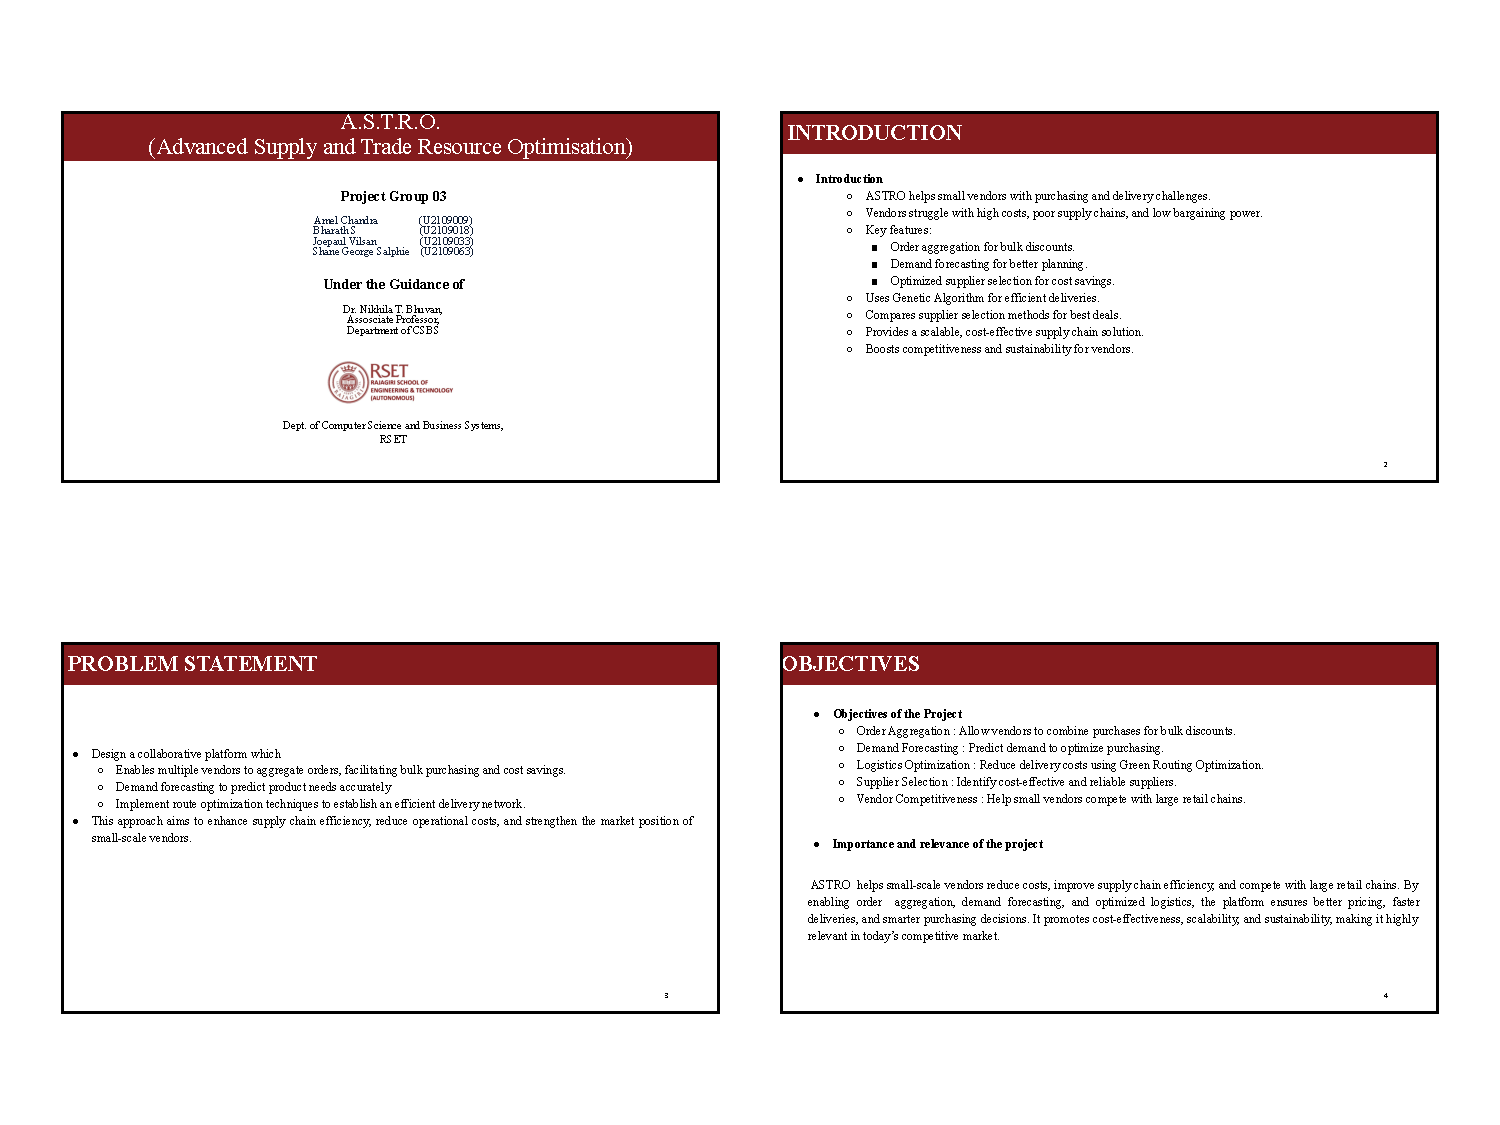
\includepdf[pages=-]{Appendices/GRP_3.pdf}

\clearpage
\addcontentsline{toc}{chapter}{Appendix B: Vision, Mission, PO, PSO, and CO}
\chapter*{}
\paragraph\
\vspace{75mm}
\begin{center}
	\textbf{\huge{Appendix B: }}
	\textbf{\huge{Vision, Mission, PO, PSO, and CO}}
\end{center}
%	\includepdf[pages=-]{2.pdf}
\clearpage
\clearpage
\newpage
%\cleardoublepage
\thispagestyle{empty}
\begin{center}
	\Large \bfseries RAJAGIRI SCHOOL OF ENGINEERING AND TECHNOLOGY (AUTONOMOUS)
\end{center}
\vspace{0.5cm}
\renewcommand{\baselinestretch}{1.2}\normalsize
\noindent\textbf{Vision}
\begin{tcolorbox}[colback=white, colframe=black, rounded corners, width=\textwidth]
	To evolve into a premier technological and research institution, molding eminent professionals with creative minds, innovative ideas and sound practical skill, and to shape a future where technology works for the enrichment of mankind.
\end{tcolorbox}

\noindent\textbf{Mission}
\begin{tcolorbox}[colback=white, colframe=black, rounded corners, width=\textwidth]
	To impart state-of-the-art knowledge to individuals in various technological disciplines and to inculcate in them a high degree of social consciousness and human values, thereby enabling them to face the challenges of life with courage and conviction.
\end{tcolorbox}

\vspace{1.5cm}
\begin{center}
	\Large \bfseries DEPARTMENT OF COMPUTER SCIENCE AND BUSINESS SYSTEMS
\end{center}
\vspace{0.5cm}
\noindent\textbf{Vision}
\begin{tcolorbox}[colback=white, colframe=black, rounded corners, width=\textwidth]
	To evolve into a department of excellence in information technology by the creation and exchange of knowledge through leading-edge research, innovation and services, which will in turn contribute towards solving complex societal problems and thus building a peaceful and prosperous mankind.
\end{tcolorbox}

\noindent\textbf{Mission}
\begin{tcolorbox}[colback=white, colframe=black, rounded corners, width=\textwidth]
	To impart high-quality technical education, research training, professionalism and strong ethical values in the young minds for ensuring their productive careers in industry and academia so as to work with a commitment to the betterment of mankind.

\end{tcolorbox}


%	To inspire and nurture students, with up-to-date knowledge in Computer Science and Engineering, ethics, team spirit, leadership abilities, innovation and creativity to come out with solutions meeting societal needs. \\ \\
\newpage
\noindent\textbf{Programme Outcomes (PO)} \\
Engineering Graduates will be able to:
\begin{enumerate}
	\item {Engineering Knowledge:} Apply the knowledge of mathematics, science, engineering fundamentals, and an engineering specialization to the solution of complex engineering problems.
	\item {Problem Analysis:} Identify, formulate, review research literature, and analyze complex engineering problems reaching substantiated conclusions using first principles of mathematics, natural sciences, and engineering sciences.
	\item {Design/Development of Solutions:} Design solutions for complex engineering problems and design system components or processes that meet the specified needs with appropriate consideration for public health and safety, and the cultural, societal, and environmental considerations.
	\item {Conduct Investigations of Complex Problems:} Use research-based knowledge including design of experiments, analysis and interpretation of data, and synthesis of the information to provide valid conclusions.
	\item {Modern Tool Usage:} Create, select, and apply appropriate techniques, resources, and modern engineering and IT tools including prediction and modeling to complex engineering activities with an understanding of the limitations.
	\item {The Engineer and Society:} Apply reasoning informed by the contextual knowledge to assess societal, health, safety, legal, and cultural issues and the consequent responsibilities relevant to the professional engineering practice.
	\item {Environment and Sustainability:} Understand the impact of the professional engineering solutions in societal and environmental contexts, and demonstrate the knowledge of, and need for sustainable development.
	\item {Ethics:} Apply ethical principles and commit to professional ethics and responsibilities and norms of the engineering practice.
	\item {Individual and Team Work:} Function effectively as an individual, and as a member or leader in teams, and in multidisciplinary settings.
	\item {Communication:} Communicate effectively on complex engineering activities with the engineering community and with society at large, such as, being able to comprehend and write effective reports and design documentation, make effective presentations, and give and receive clear instructions.
	\item {Project Management and Finance:} Demonstrate knowledge and understanding of engineering and management principles and apply these to one’s own work, as a member and leader in a team. Manage projects in multidisciplinary environments.
	\item {Life-long Learning:} Recognize the need for, and have the preparation and ability to engage in independent and lifelong learning in the broadest context of technological change.
\end{enumerate}

\subsection*{Programme Specific Outcomes (PSO)}

A graduate of the Computer Science and Business Systems Programme will:
\begin{itemize}
	\item \textbf{PSO 1: Programming and Software Development Skills} \\
	      Demonstrate ability to analyze, design, and implement software solutions incorporating various programming concepts.
	\item \textbf{PSO 2: Engineering Management and Collaboration} \\
	      Comprehend professional, managerial, and financial aspects of business and collaborate on the design, implementation, and integration of engineering solutions.
	\item \textbf{PSO 3: Decision-Making and Analytical Techniques in Engineering and Business} \\
	      Create, select, and apply appropriate techniques and business tools, including prediction and data analytics, for complex engineering activities and business solutions.
\end{itemize}

\subsection*{Course Outcomes (CO)}

After successful completion of the course, the students will be able to:
\begin{itemize}
	\item {CO1:} Model and solve real-world problems by applying knowledge across domains (Cognitive knowledge level: Apply).
	\item {CO2:} Develop products, processes, or technologies for sustainable and socially relevant applications (Cognitive knowledge level: Apply).
	\item {CO3:} Function effectively as an individual and as a leader in diverse teams and to comprehend and execute designated tasks (Cognitive knowledge level: Apply).
	\item {CO4:} Plan and execute tasks utilizing available resources within timelines, following ethical and professional norms (Cognitive knowledge level: Apply).
	\item{CO5:} Identify technology/research gaps and propose innovative/creative solutions (Cognitive knowledge level: Analyze).
	\item {CO6:} Organize and communicate technical and scientific findings effectively in written and oral forms (Cognitive knowledge level: Apply).
\end{itemize}
\addcontentsline{toc}{chapter}{Appendix C: CO-PO-PSO Mapping}
\chapter*{}
\paragraph\
\vspace{75mm}
\begin{center}
    \textbf{\huge{Appendix B: }}
    \textbf{\huge{CO-PO-PSO Mapping}}
\end{center}
%	\includepdf[pages=-]{2.pdf}
\clearpage
\clearpage
\newpage
%\cleardoublepage
\thispagestyle{empty}

\begin{table}[htp]
    \centering
    \caption*{Mapping of Course Outcomes (CO) with Programme Outcomes (PO)}
    \scalebox{0.8}{
        \begin{tabular}{|c|c|c|c|c|c|c|c|c|c|c|c|c|}
            \hline
            \textbf{}     & \textbf{PO 1} & \textbf{PO 2} & \textbf{PO 3} & \textbf{PO 4} & \textbf{PO 5} & \textbf{PO 6} & \textbf{PO 7} & \textbf{PO 8} & \textbf{PO 9} & \textbf{PO 10} & \textbf{PO 11} & \textbf{PO 12} \\ \hline
            \textbf{CO 1} & 2             & 2             & 2             & 1             & 2             & 2             & 2             & 1             & 1             & 1              & 1              & 2              \\ \hline
            \textbf{CO 2} & 2             & 2             & 2             &               & 1             & 3             & 3             & 1             & 1             &                & 1              & 1              \\ \hline
            \textbf{CO 3} &               &               &               &               &               &               &               &               & 3             & 2              & 2              & 1              \\ \hline
            \textbf{CO 4} &               &               &               &               & 2             &               &               & 3             & 2             & 2              & 3              & 2              \\ \hline
            \textbf{CO 5} & 2             & 3             & 3             & 1             & 2             &               &               &               &               &                &                & 1              \\ \hline
            \textbf{CO 6} &               &               &               &               & 2             &               &               & 2             & 2             & 3              & 1              & 1              \\ \hline
        \end{tabular}}
\end{table}
\begin{table}[htp]
    \centering
    \caption*{Mapping of Course Outcomes (CO) with Programme Specific Outcomes (PSO)}
    \begin{tabular}{|c|c|c|c|}
        \hline
        \textbf{}     & \textbf{PSO 1} & \textbf{PSO 2} & \textbf{PSO 3} \\ \hline
        \textbf{CO 1} & 3              & 1              & 2              \\ \hline
        \textbf{CO 2} & 3              & 3              & 2              \\ \hline
        \textbf{CO 3} &                & 3              &                \\ \hline
        \textbf{CO 4} &                & 1              & 1              \\ \hline
        \textbf{CO 5} & 1              & 1              & 1              \\ \hline
        \textbf{CO 6} &                & 2              &                \\ \hline
    \end{tabular}
\end{table}
%\clearpage

\end{document}